\documentclass[]{article}
\usepackage[pdftex]{graphicx}  
\begin{document}

\begin{enumerate}

\item Figure \ref{dogigree} is a pedigree of miniature schnauzers (a dog breed). Female \#2 has already had one litter, and male \#3 has already sired two offspring with female \#4. A breeder is interested in mating female \#2 and male \#3, but is worried about Von-Willibrands disease in their offspring. The breeder had female \#2 tested for the disease, and the test result suggested she was a carrier. The test is imperfect, however, and ~20\% of the time returns an incorrect positive result. You are a geneticist brought in to advise the breeder. Answer the following:

\begin{enumerate}
\item What are the genotypes of dogs \#1, \#3, and \#4? (6pts)
\item What is the most likely genotype of dog \#2? Explain how you reach this conclusion. (6pts)
\item Given the genotypes above, what is the probability that dogs \#2 and \#3 will have: (4 pts)
\begin{enumerate}
\item A male puppy with Von-Willibrands disease?
\item A female puppy with Von-Willibrands disease?
\item A normal female puppy?
\item A normal male puppy?
\end{enumerate}
\end{enumerate}

%-------------------------------------------------------------------
\begin{figure*}[h]
  \begin{center}
   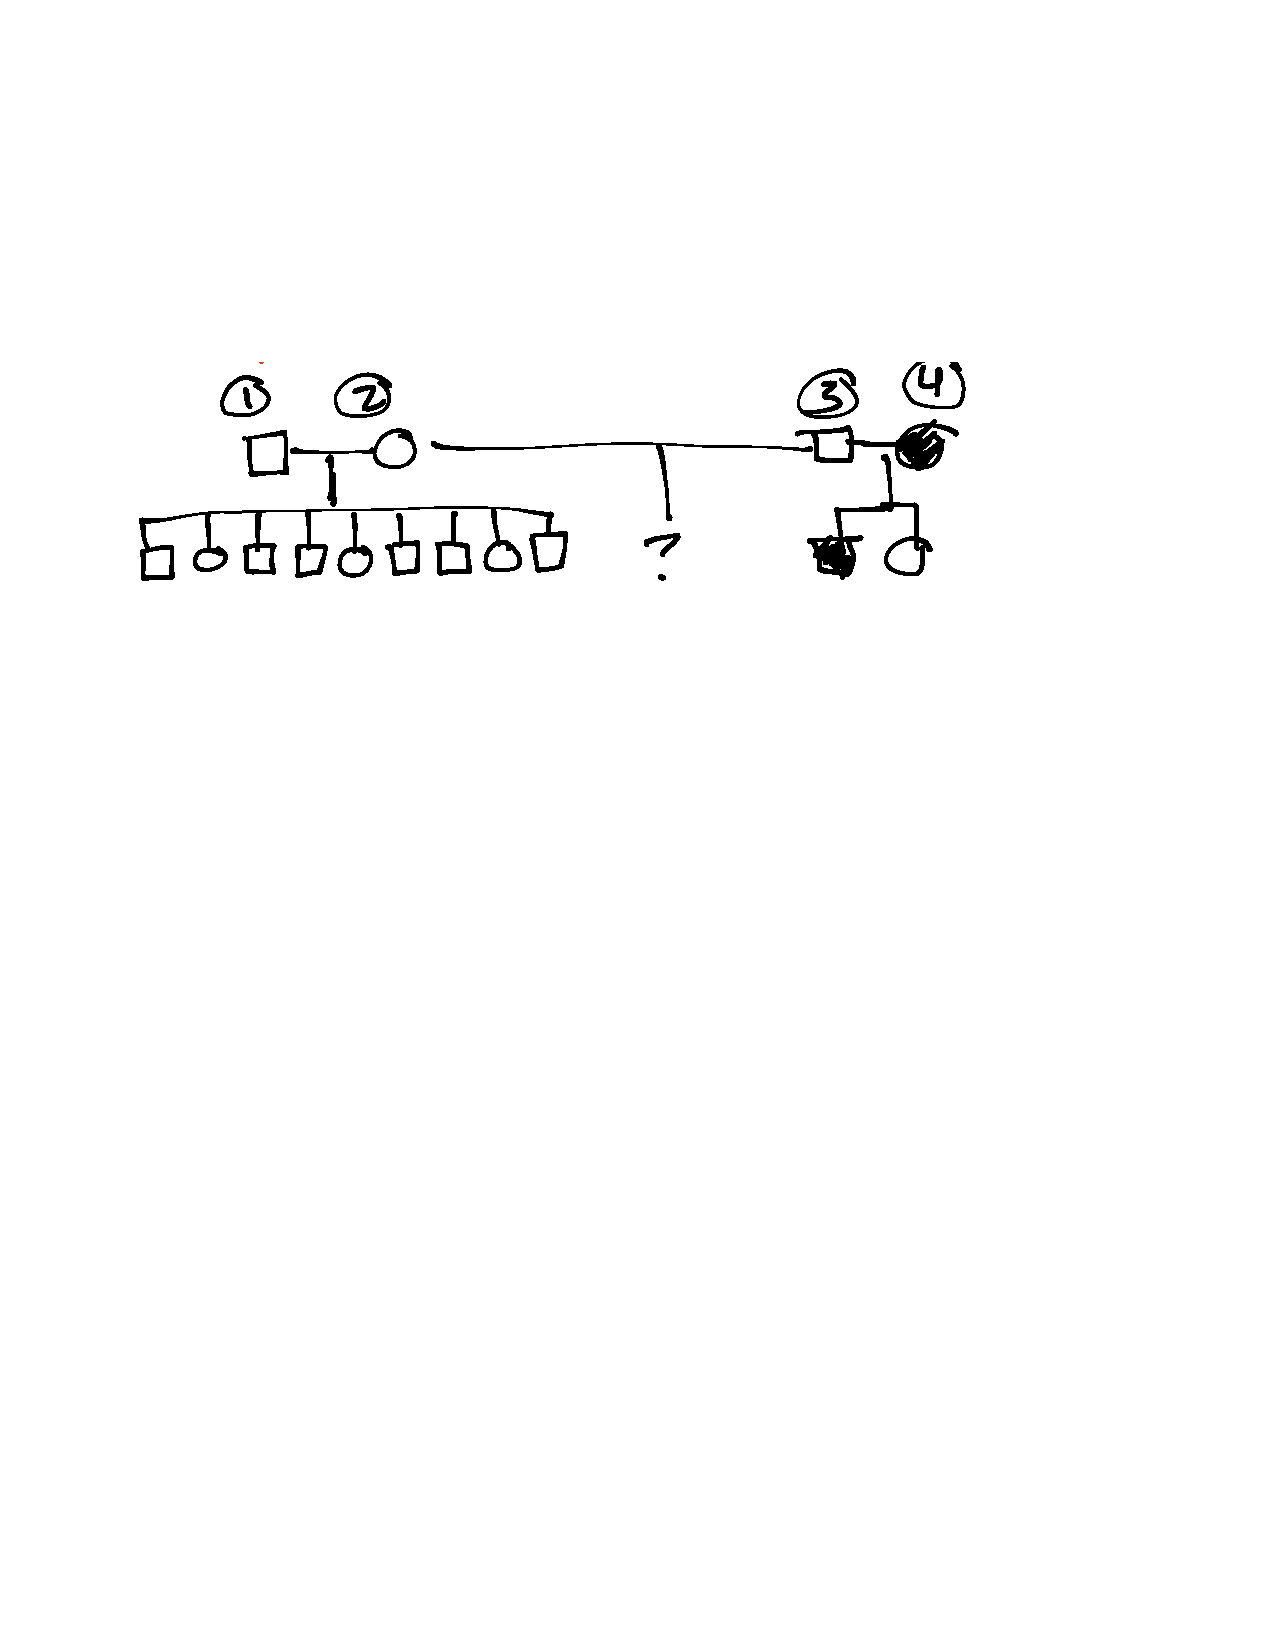
\includegraphics[width=130mm]{/Users/jri/src/bis101/images/pedigree_test.pdf}
\label{dogigree}
\caption{A pedigree of miniature schnauzers. Filled symbols (square=male, circle=female) represent dogs with Von-Willibrands disease, a recessive X-linked disorder. Empty symbols are dogs with wild-type phenotypes.}
  \end{center}
\end{figure*}
%-------------------------------------------------------------------

\end{enumerate}

\end{document}